\section{Analysis tasks}
\label{sec:analysis-tasks}

In this section, we study a range of fundamental analysis tasks, namely function reconstruction
(Section~\ref{sec:rmse-optimized}), gradient computation (Section~\ref{sec:gradient}), Laplacian
computation (Section~\ref{sec:laplacian}), histogram computation (Section~\ref{sec:histogram}), and
isocontour extraction (Section~\ref{sec:isocontour}). For each task, we define an error metric $E$
(see Section~\ref{sec:data_dep_streams}) that is the basis for evaluating a stream's performance.
Algorithm~\ref{alg:greedy} is used to compute a greedy stream optimized for the task at hand, in
terms of minimizing the relevant $E$ at every point. Each analysis task potentially requires a
fundamentally different stream for optimal results. Therefore, the goal is to distill the core
characteristics of these optimized streams. To accomplish this goal, we define and make use of a
concept named \emph{stream signature} (Section~\ref{sec:stream-signature}). The signature of a
stream is a small matrix that encodes the stream's ``preferences'' in terms of
precision-versus-resolution tradeoffs. As such, the signature not only reveals the characteristics
of a stream, but can also be used in practice to ``steer'' streaming in a way that is optimized for
the task at hand.

\subsection{Stream signatures}
\label{sec:stream-signature}

To analyze the core characteristics of a stream, we introduce the concept of a \emph{stream
signature}. A signature is a $\bar{l} \times \bar{b}$ matrix, with $\bar{b}$ being the number of bit
planes, and $\bar{l}$ the number of wavelet subbands. The $(l,b)$ element of the matrix is
associated with chunks belonging in subband $l$ and bit plane $b$ , and contains an integer value in
the range $[0,\bar{b}\times \bar{l})$. This value indicates, on average, the position in which
chunks associated with that element appear in the stream, relative to chunks associated with other
elements. For example, the signature  $A=\bigl[
\begin{smallmatrix}0 & 1 & 4\\ 2 & 3 & 5\end{smallmatrix}\bigr]$ conveys the information that the
most important chunks lie on the first bit plane of the first subband ($A_{0,0}=0$), followed by
chunks lying on the second bit plane of the first subband ($A_{0,1}=1$), then the first bit plane of
the second subband ($A_{1,0}=2$), and so on.

To compute a stream signature, we partition the whole domain into several \emph{regions}, compute
one signature per region, then sum all the per-region signatures. Partitioning is needed since it is
only meaningful to compute the relative ordering of chunks if they come from the the same (``small''
enough) region. For example, a chunk at one corner of the domain can be streamed before another
chunk at an opposite corner, but this fact contains no useful information. We want a region to be as
small as possible, and define a region to be the spatial volume/area that is covered by a chunk in
the coarsest subband. So, the total number of regions, $\bar{r}$, is the same as the number of
chunks in the coarsest subband. Note that regions exist in the global domain, as they are not
confined to individual subbands. Ideally, the global signature should retain information from all
the per-region signatures, but due to space constraints, we have chosen to condense all the local
signatures by summing them into one signature. This choice results in signatures that are less
meaningful for data that contains a high degree of spatial variability. We have found, however, that
this choice works well for the various data sets used in this paper. If signatures are deemed useful
enough to be deployed in practice, a more sophisticated ``compression'' of the signature stack might
be necessary for the best results.

The following algorithm computes a stream signature.

\begin{algorithm}[h]
  \caption{Computing a stream signature}
  \begin{algorithmic}[1]
    \Inputs{
			A stream $C=\{c_i\}, i\in\{0,\dots,n-1\}$\\}
		\Initialize{Per-region signature matrix $A_r\gets 0, r\in\{0,\dots\bar{r}-1\}$\\
		Global signature matrix $A \gets 0$}
		\For{each chunk $c_i$}
			\State Let $r$, $b$, $l$ be the region, bit plane, and subband that $c_i$ belongs
			\State $A_r(l,b) \gets A_r(l,b)+i$
		\EndFor
		\For{each region $r$}
			\State Sort the elements of $A_r$
			\State Assign each element of $A_r$ its index after sorting
			\State $A \gets A+A_r$
		\EndFor
		\State Sort the elements of $A$
		\State Assign each element of $A$ its index after sorting
		\Output{The signature matrix $A$}
	\end{algorithmic}
	\label{alg:greedy}
\end{algorithm}

TODO: example signatures for the by bit plane, by level, by wavelet norm

\subsection{Function reconstruction}
\label{sec:rmse-optimized}

The most fundamental task is that of reconstructing the function itself (i.e., $Q$ is the identity
map), using a common error metric such as the root-mean-square error (RMSE). For each data set, we
use the aforementioned $O(n)$ greedy algorithm to construct an \emph{rmse-optimized} stream. In
Section \ref{sec:motivation} we have seen that the \emph{by wavelet norm} performs the best among
the data-agnostic streams with regards to RMSE. To see how the \emph{rmse-optimized} stream, which
is data-dependent, compares to the data-agnostic streams, we plot all four streams together in
Figure \ref{fig:rmse-optimized}. It can be seen that the difference between \emph{by wavelet norm}
and \emph{rmse-optimized} is negligible in most cases. This result is expected, because \emph{by
wavelet norm} and \emph{rmse-optimized} both order the chunks according to their contribution to in
the $L_2$ sense, with \emph{rmse-optimized} also taking into account the actual values of the bits.
This difference has little effect in this case, because, as leading zero bits are removed, the rest
of the bits (of the wavelet coefficients) are known to be distributed approximately uniformly among
$0$ and $1$ for wavelet coefficients [CITE]. 

Among the static streams, \emph{by level} performs poorly compared to \emph{by bit plane} and
\emph{by wavelet norm}. This is because, in the $L_2$ norm, low-ordered bits or coarse-level
coefficients contribute little compared to high-ordered bits of fine-level coefficients. This
difference in contribution is magnified when the data contains fine-scale features, as is the case
for the \emph{plasma} data set. In Figure \ref{fig:rmse-rendering}, we render this field at 0.74
bits per sample for all three streams, and compare these rendering with that of the groundtruth
data. \emph{by level} results in heavy artifacts that are not seen by \emph{by bit plane} and
\emph{by wavelet norm}. \emph{by wavelet norm} performs slightly better than \emph{by bit plane}
here and in all other cases. These results suggest that in practice, \emph{by wavelet norm} is a
near-optimal way to stream data that minimizes root-mean-square errors, regardless of the data.

\begin{figure}[h]
  \centering
	\subcaptionbox{Boiler}
  {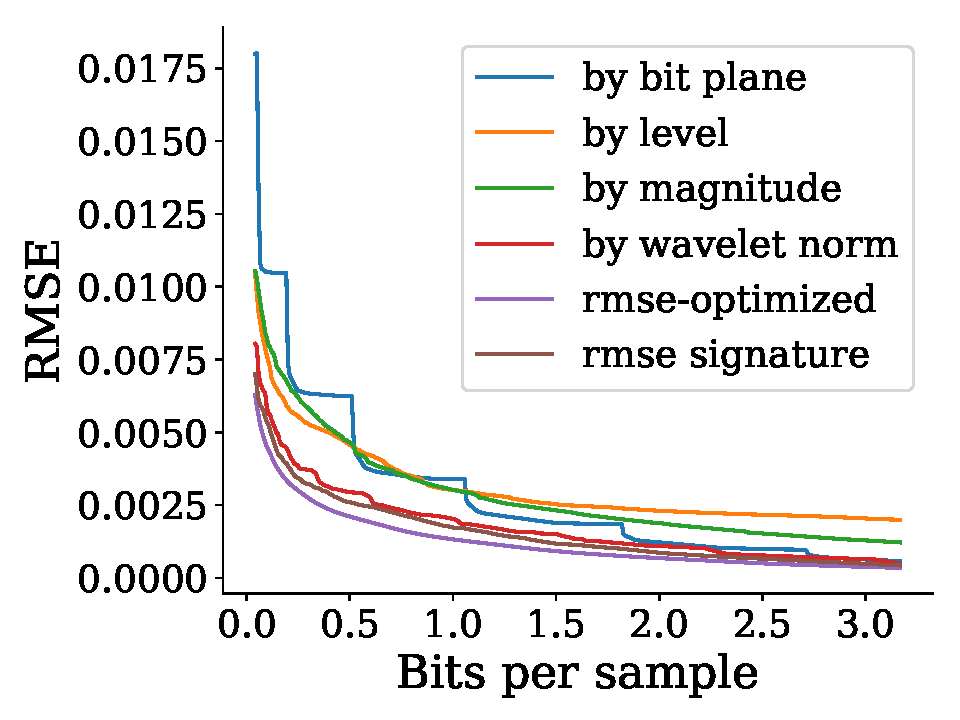
\includegraphics[width=0.48\linewidth]{img/rmse/rmse-optimized-boiler.pdf}}
	\subcaptionbox{Diffusivity}
 	{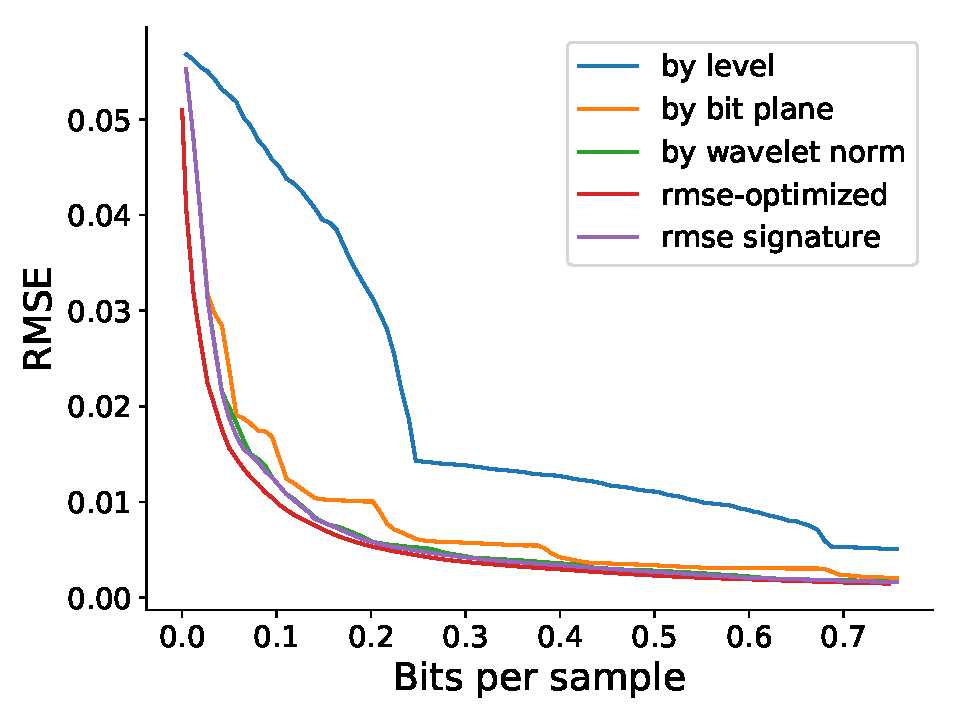
\includegraphics[width=0.48\linewidth]{img/rmse/rmse-optimized-diffusivity.pdf}}
	\subcaptionbox{Euler}
 	{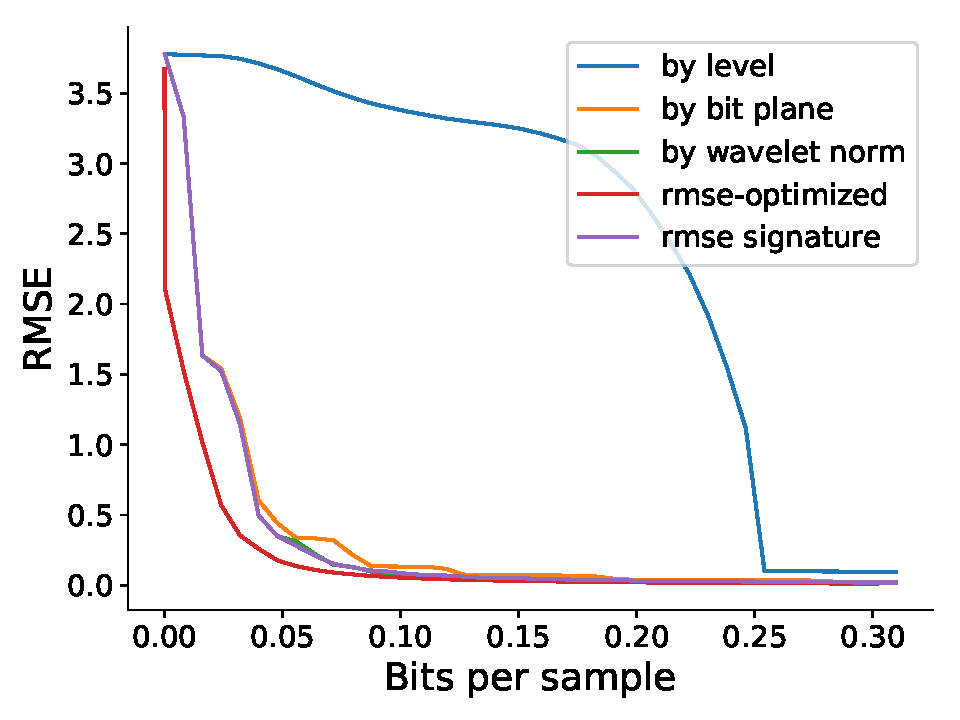
\includegraphics[width=0.48\linewidth]{img/rmse/rmse-optimized-euler.pdf}}
	\subcaptionbox{Turbulence}
 	{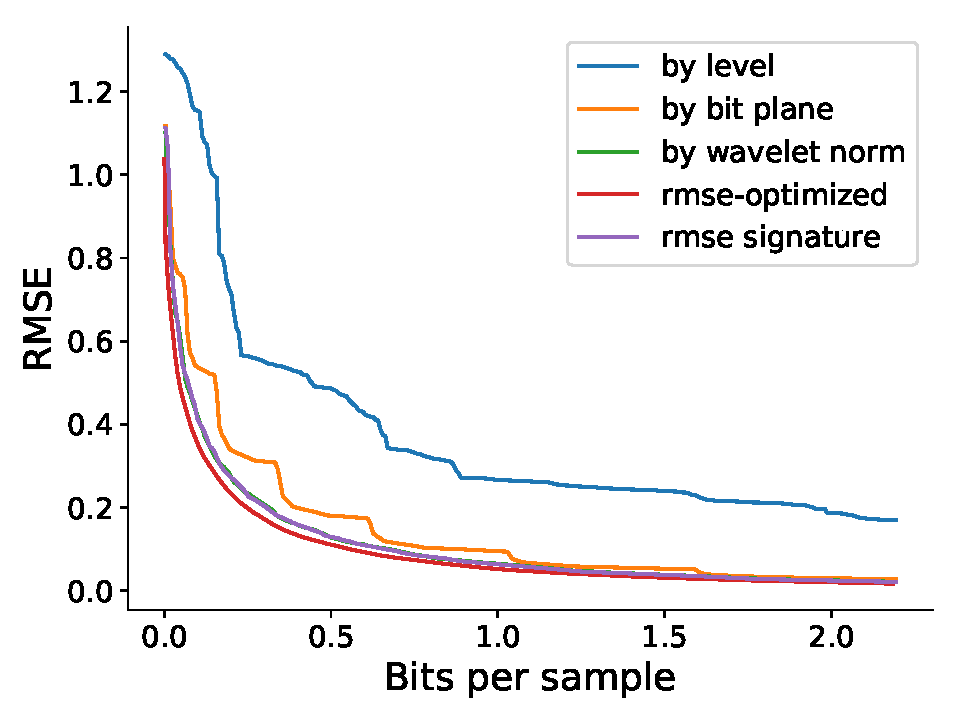
\includegraphics[width=0.48\linewidth]{img/rmse/rmse-optimized-turbulence.pdf}}
	\subcaptionbox{Plasma}
 	{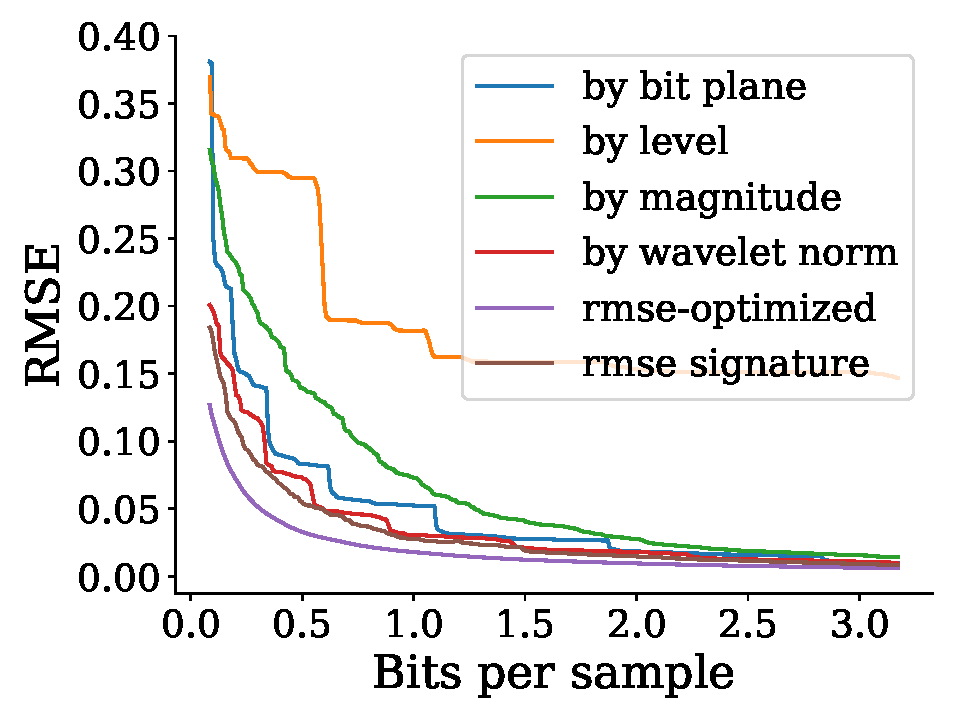
\includegraphics[width=0.48\linewidth]{img/rmse/rmse-optimized-plasma.pdf}}
	\subcaptionbox{Velocity-z}
 	{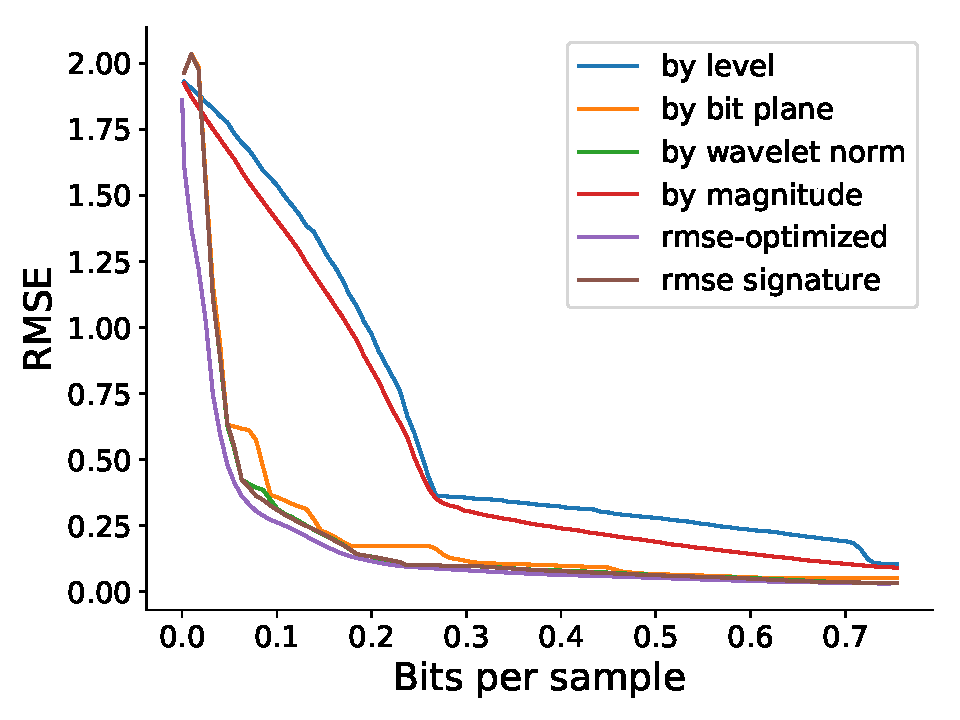
\includegraphics[width=0.48\linewidth]{img/rmse/rmse-optimized-velocityz.pdf}}
 	\caption{Root-mean-square error of reconstructed functions for the three data-agnostic streams
 	defined in Section \ref{sec:motivation}, and the \emph{rmse-optimized} stream. Lower is better.
 	The streams are truncated to highlight the differences, without omitting important information.
 	\emph{rmse-optimized} performs best, followed closely by \emph{by wavelet norm} and \emph{by bit
 	plane}.}
 	\label{fig:rmse-optimized}
\end{figure}

\begin{figure}[h]
	\centering
	{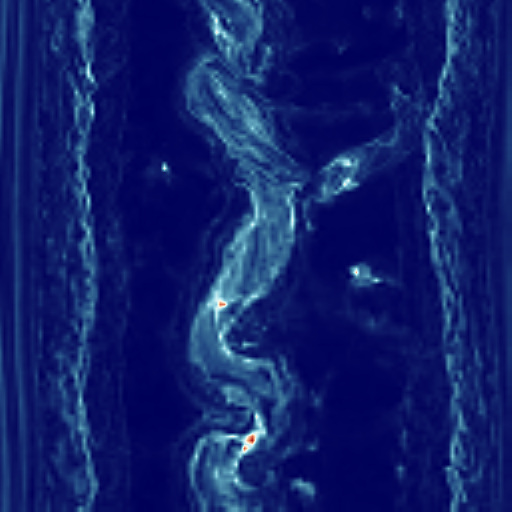
\includegraphics[width=0.24\linewidth]{img/rmse/plasma_curr_func2.png}}
	{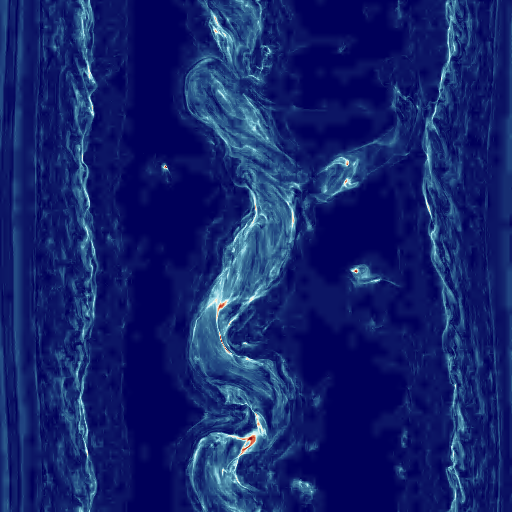
\includegraphics[width=0.24\linewidth]{img/rmse/plasma_curr_func1.png}}
	{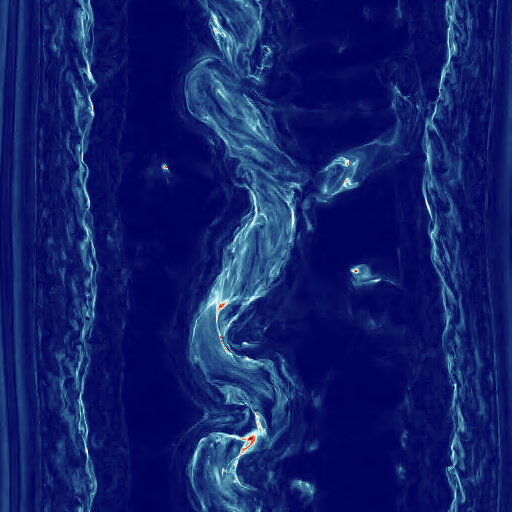
\includegraphics[width=0.24\linewidth]{img/rmse/plasma_curr_func0.png}}
	{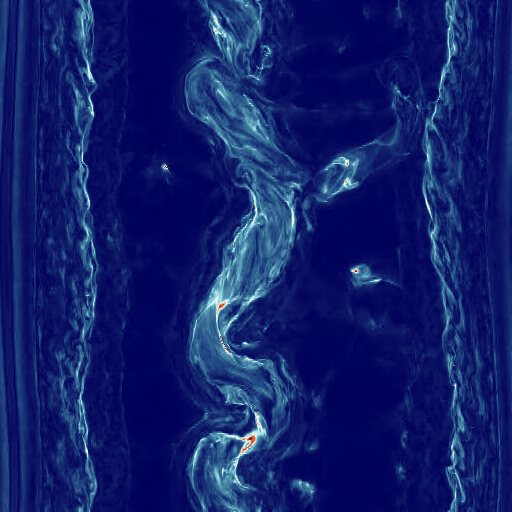
\includegraphics[width=0.24\linewidth]{img/rmse/signature_curr_func0.png}}
	{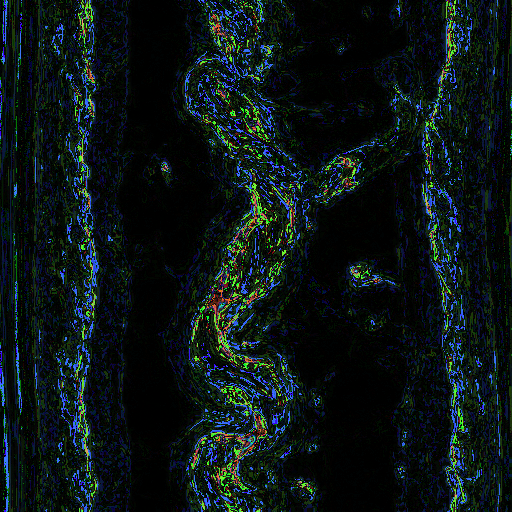
\includegraphics[width=0.24\linewidth]{img/rmse/plasma_curr_func2_diff.png}}
	{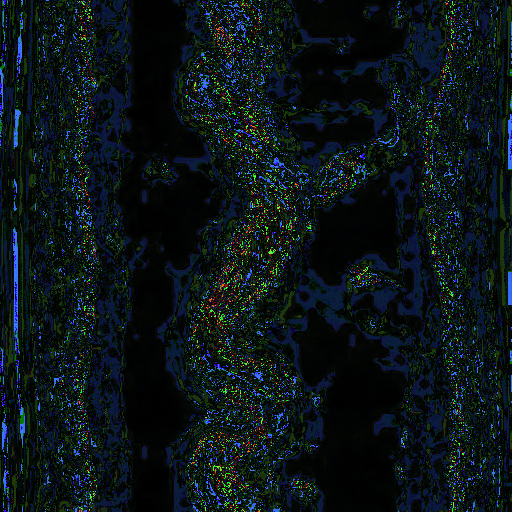
\includegraphics[width=0.24\linewidth]{img/rmse/plasma_curr_func1_diff.png}}
	{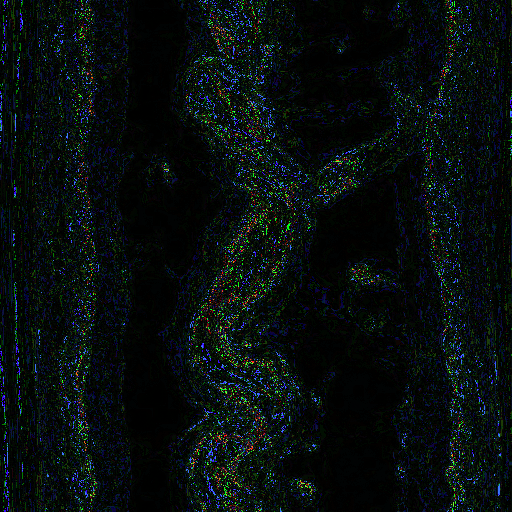
\includegraphics[width=0.24\linewidth]{img/rmse/plasma_curr_func0_diff.png}}
	{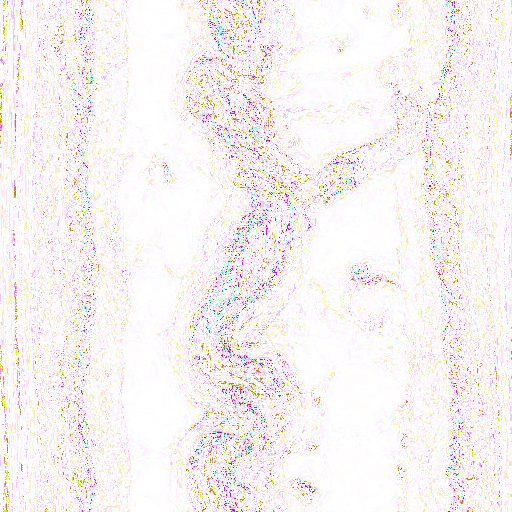
\includegraphics[width=0.24\linewidth]{img/rmse/signature_curr_func0_diff.png}}
	
	\caption{Top row:	renderings of the \emph{plasma} function at 0.74 bps. From left to right:
	\emph{by level}, \emph{by bit plane}, \emph{by wavelet norm}, and ground-truth. Bottom row:
	difference (XOR) of the reconstructed images (in respective order) from the groundtruth image,
	brighter pixels mean higher errors. The \emph{by wavelet norm} provides the most accurate
	function, followed closely by
	\emph{by bit plane}.}
 	\label{fig:rmse-rendering}
\end{figure}

\begin{figure}[h]
	\centering
	{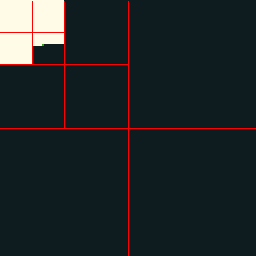
\includegraphics[width=0.24\linewidth]{img/rmse/rmse-precision-dist-by-level.png}}
	{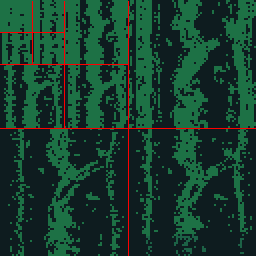
\includegraphics[width=0.24\linewidth]{img/rmse/rmse-precision-by-bit-plane.png}}
	{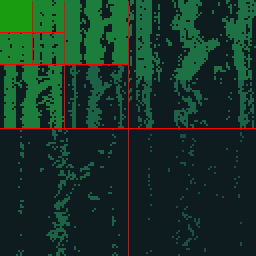
\includegraphics[width=0.24\linewidth]{img/rmse/rmse-precision-dist-by-wavelet-norm.png}}
	{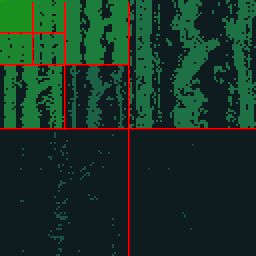
\includegraphics[width=0.24\linewidth]{img/rmse/rmse-precision-signature.png}}
	
	\caption{Precision distribution, plasma, 0.74 bps.}
 	\label{fig:rmse-rendering}
\end{figure}
